\documentclass[12pt,a4paper,UTF8]{ctexart}
\usepackage{geometry}
\geometry{left=2.5cm,right=2.5cm,top=2.5cm,bottom=2.5cm}
\usepackage{fancyhdr}
\usepackage{graphicx}
\usepackage{amsmath}
\usepackage{amssymb}
\usepackage{titlesec}
\usepackage{ulem}
\usepackage{caption}
\usepackage{enumitem}
\usepackage{parskip}
\usepackage{multirow}

% 行距
\linespread{1.25}

% 页眉页脚
\setlength{\headheight}{15pt}
\pagestyle{fancy}
\fancyhf{}
\fancyhead[C]{\small 哈尔滨工业大学（深圳）实验报告}
\fancyfoot[C]{\thepage}
\renewcommand{\headrulewidth}{0.4pt}

% 标题格式
\titleformat{\section}{\bfseries\zihao{4}}{}{0em}{}
\titleformat{\subsection}{\bfseries\zihao{-4}}{}{0em}{}
\titleformat{\subsubsection}{\bfseries\zihao{-4}}{}{0em}{}

% 列表设置
\setlist[itemize]{leftmargin=*}
\setlist[enumerate]{leftmargin=*}

\begin{document}

% -------------------------- 封面 --------------------------
\begin{titlepage}
    \centering
    \vspace*{2cm}
    
\includegraphics[height=3.0cm]{logo.png}\\[0.5cm]
    {\heiti\zihao{3} 哈尔滨工业大学（深圳）}\\[0.3cm]
    {\small \textit{Harbin Institute of Technology, Shenzhen}}
    
    \vspace{3cm}
    {\heiti\zihao{1} 实验报告}\\[0.3cm]
    \rule{8cm}{1pt}\\[0.3cm]
    
    \vspace{2cm}
    \begin{minipage}{13cm}
    \zihao{4}
    \renewcommand{\arraystretch}{1.8}
    \begin{tabular}{ll}
    课程名称： & \uline{\quad 自动控制理论 \hfill} \\
    学生姓名： & \uline{\quad 余泓彬 \hfill} \\
    班级学号： & \uline{\quad 2024312506 \hfill} \\
    学生专业： & \uline{\quad 电气工程及其自动化 \hfill} \\
    实验名称： & \uline{\quad 实验四 PID模拟控制器综合设计 \hfill} \\
    报告时间： & \uline{\quad 2026-05-29 \hfill}
    \end{tabular}
    \end{minipage}
    
    \vfill
    {\zihao{4} 哈尔滨工业大学（深圳）}
    \vspace{1.5cm}
\end{titlepage}

% -------------------------- 正文 --------------------------
\clearpage
\setcounter{page}{1}

\section{实验四·PID模拟控制器综合设计}

\subsection{一、实验目的}
\begin{enumerate}
    \item 设计系统超前校正装置，分析校正环节对控制系统动态、稳态性能的影响。
    \item 深入理解P/PI/PD控制规律机理，掌握频域校正设计思路。
    \item 能够运用频率特性法针对已知数学模型的被控对象完成控制器参数工程设计与实物验证。
\end{enumerate}

\subsection{二、实验设备及元器件}
\begin{enumerate}
    \item PC 机一台（预装MATLAB、NI ELVIS上位采集软件）
    \item NI ELVIS III 测控实验平台一台
    \item ``Circuits Control Board - 2''自动控制原理模拟实验板
    \item 配套信号连接线、分立电阻电容元器件若干
\end{enumerate}

\subsection{三、实验原理及实验过程}
\paragraph{说明：}简述实验原理，推导有关公式，结合控制器设计指标完成仿真与模拟电路搭建，相关计算与仿真结果录入报告。

\subsubsection{3.1 PID 控制器的形式}
PID 控制器有三种常用表达形式：
\begin{itemize}
    \item \textbf{零极点形式：}
    \[
    G_{\text{PID}}(s) = \frac{K_1(s+z_1)(s+z_2)}{s}
    \]
    其中：$-z_1$、$-z_2$ 分别为控制器两个零点。

    \item \textbf{时间常数形式：}
    \[
    G_{\text{PID}}(s) = \frac{K(\tau_1 s+1)(\tau_2 s+1)}{s}
    \]

    \item \textbf{PID 参数形式：}
    \[
    G_{\text{PID}}(s) = K_{\text{P}} + \frac{K_{\text{I}}}{s} + K_{\text{D}} s
    \]
\end{itemize}

\textbf{(1) 推导零点、时间常数与 PID 系数的关系。}

将零极点形式整式展开：
\[
G_{\text{PID}}(s) = \frac{K_1(s+z_1)(s+z_2)}{s}
= K_1 s + K_1(z_1+z_2) + \frac{K_1 z_1 z_2}{s}
\]
与标准PID参数表达式逐项对比可得系数关系：
\[
\begin{cases}
K_{\text{D}} = K_1 \\
K_{\text{P}} = K_1(z_1+z_2) \\
K_{\text{I}} = K_1 z_1 z_2
\end{cases}
\]

同理，将时间常数形式展开并整理对比：
\[
\begin{cases}
K_{\text{D}} = K\tau_1\tau_2 \\
K_{\text{P}} = K(\tau_1+\tau_2) \\
K_{\text{I}} = K
\end{cases}
\]

\textbf{(2) 写出 PI 控制器的三种形式。}
\begin{itemize}
    \item \textbf{零极点形式：} 
    \[G_{\text{PI}}(s) = \frac{K_1(s+z_1)}{s}\]
    \item \textbf{时间常数形式：} 
    \[G_{\text{PI}}(s) = \frac{K(\tau_1 s+1)}{s}\]
    \item \textbf{PI 参数形式：} 
    \[G_{\text{PI}}(s) = K_{\text{P}} + \frac{K_{\text{I}}}{s}\]
\end{itemize}

\textbf{(3) 说明比例、积分和微分的控制作用。}
\begin{itemize}
    \item \textbf{比例控制（P）：}快速跟随系统偏差、减小稳态误差，但比例增益过大易引发系统持续振荡。
    \item \textbf{积分控制（I）：}依靠积分累积作用消除系统阶跃稳态误差，缺点是引入相位滞后，降低系统稳定裕度。
    \item \textbf{微分控制（D）：}预判误差变化速率，提供相位超前补偿、抑制动态超调，缺点是对高频测量噪声十分敏感。
\end{itemize}

\subsubsection{3.2 PI 控制器的设计【MATLAB 仿真】}
\paragraph{(1) 频率特性设计法}
\begin{enumerate}
    \item 按照频域校正原理整定PI控制器参数，手工绘制系统开环幅频渐近折线波特图，如下图所示：
    \begin{figure}[htbp]
        \centering
        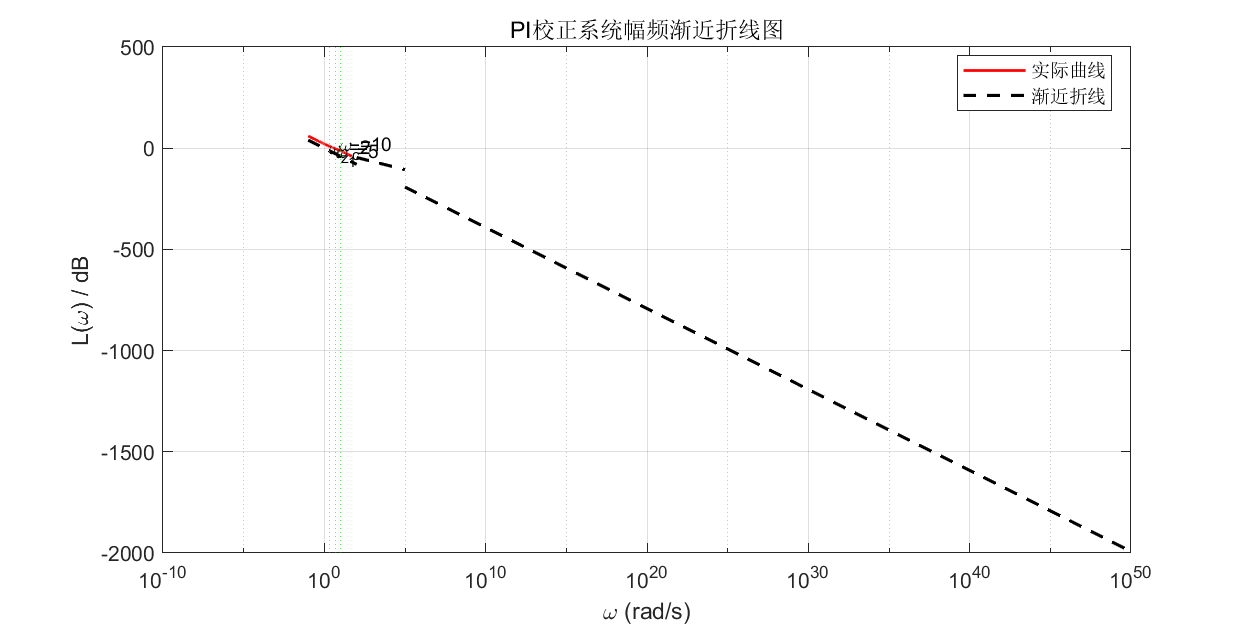
\includegraphics[width=0.7\textwidth]{3.1.png}
        \caption{PI 校正系统幅频渐近折线图}
    \end{figure}

    \item 利用MATLAB完成系统仿真，输出开环波特图与闭环阶跃响应曲线，在图中标注开环剪切频率、相角裕度，以及时域超调量、峰值时间、调节时间指标，仿真结果如下：
    \begin{figure}[htbp]
        \centering
        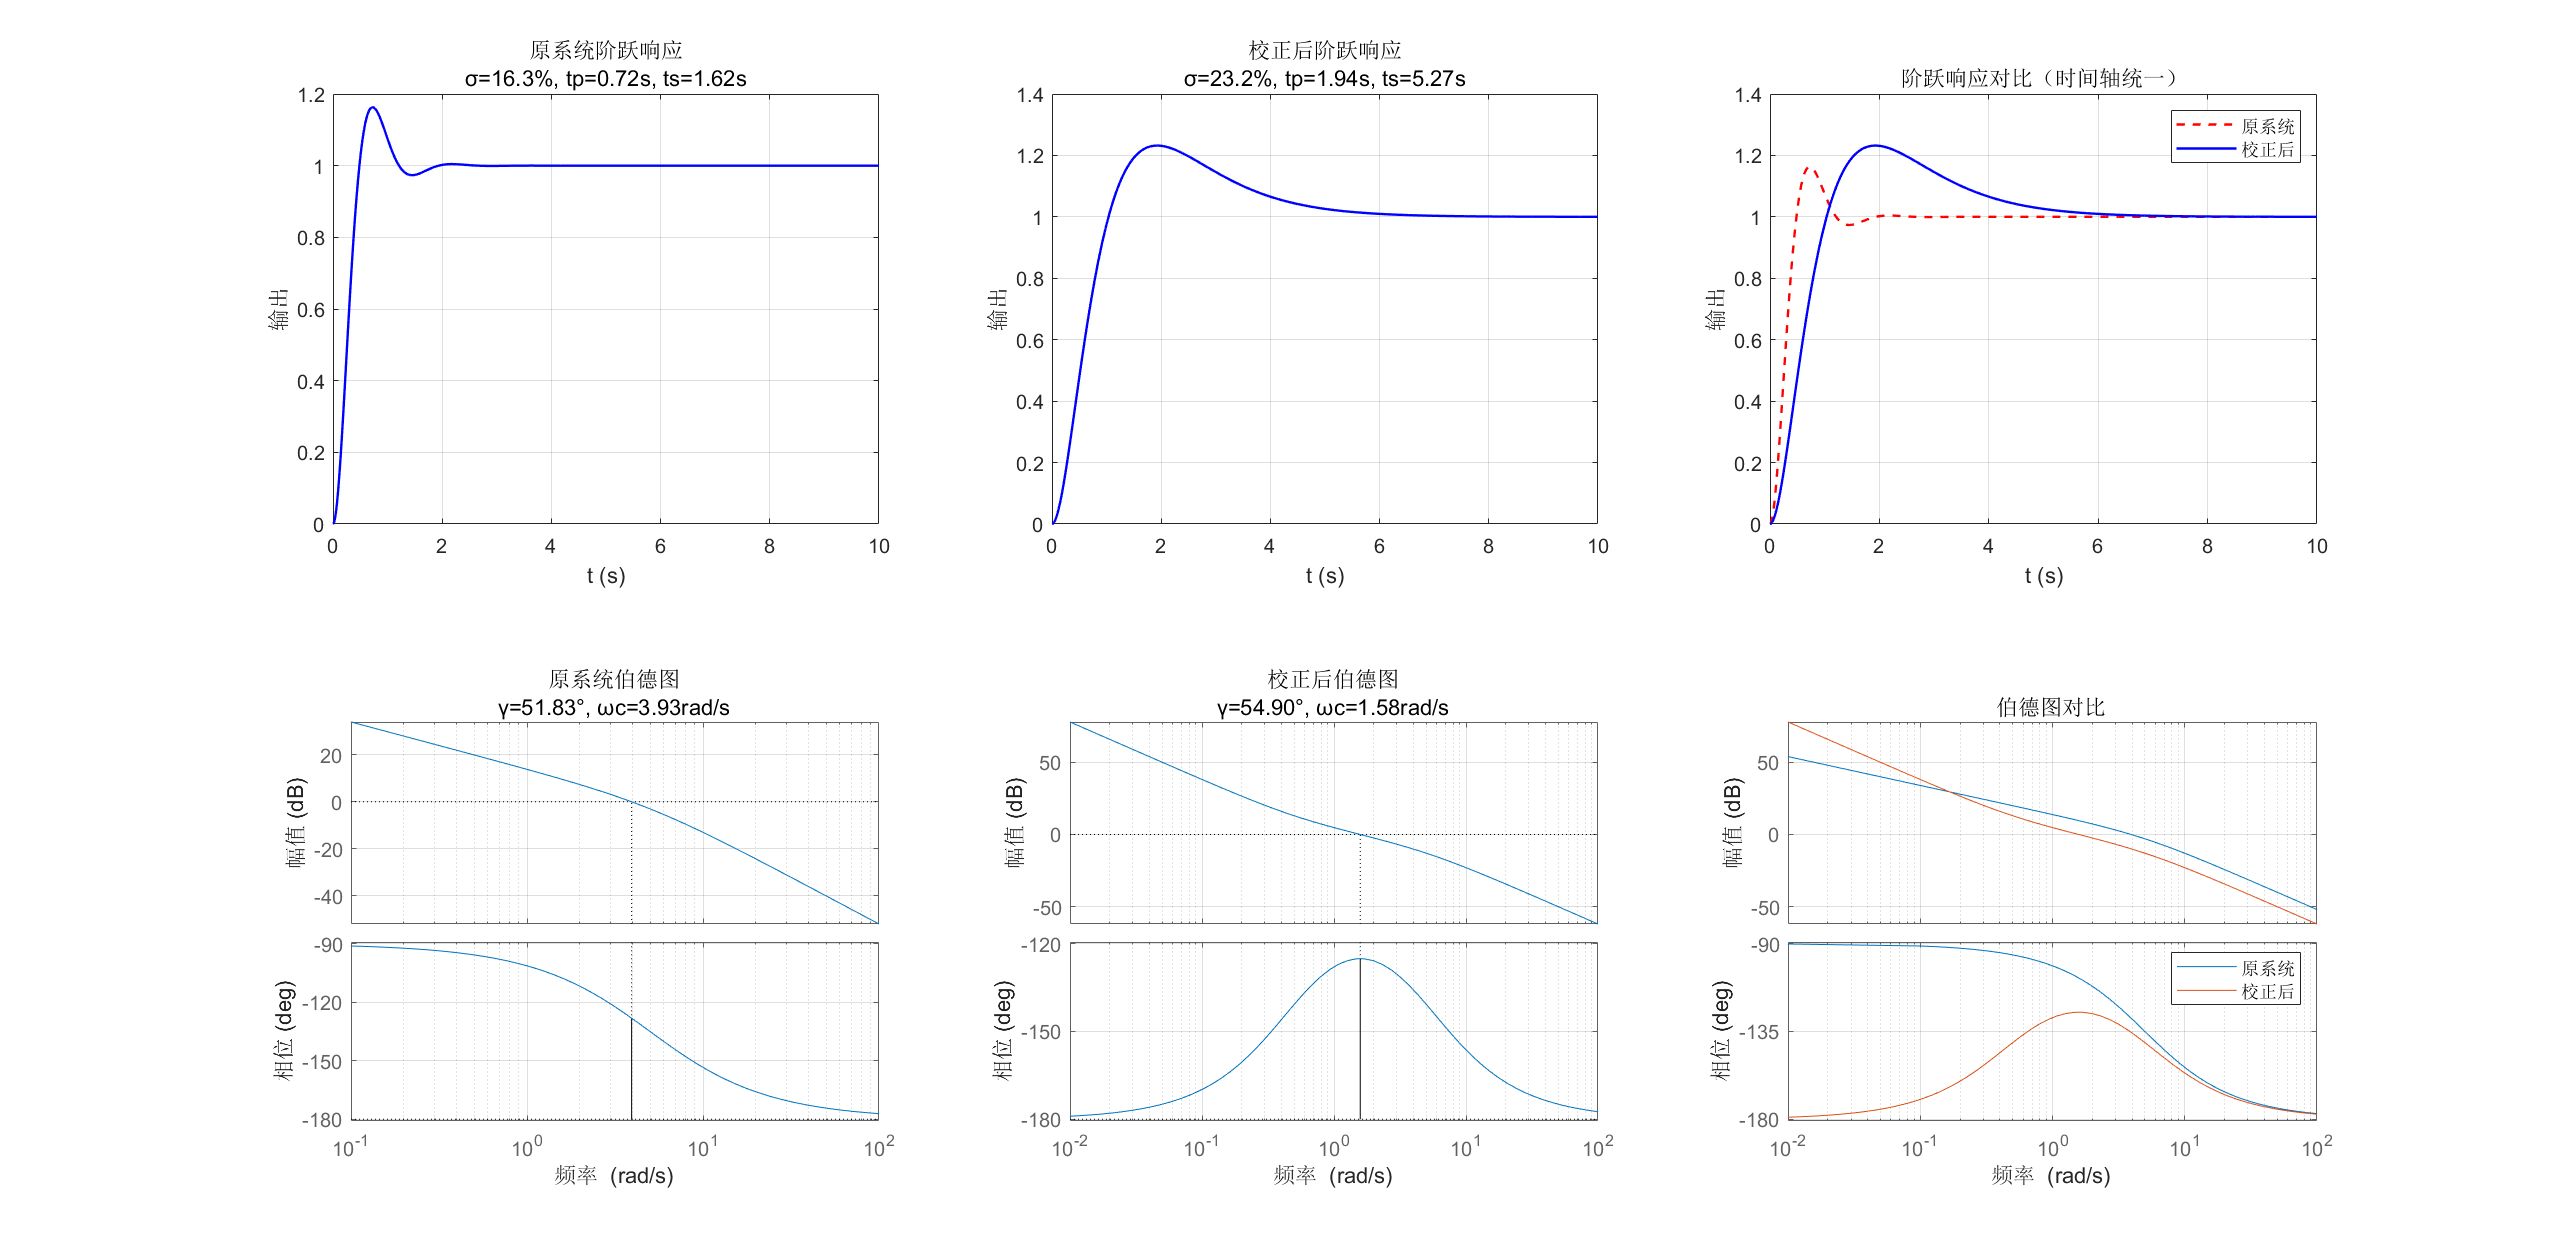
\includegraphics[width=0.7\textwidth]{3.2.png}
        \caption{MATLAB仿真：开环波特图+闭环阶跃响应曲线}
    \end{figure}
\end{enumerate}

\subsubsection{3.3 线性系统的校正}
\textbf{(1) 未校正系统}
\begin{enumerate}
    \item 未校正系统方框图
    \begin{center}
    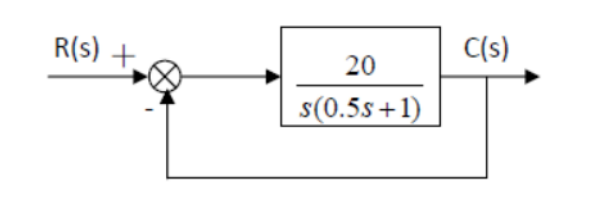
\includegraphics[width=0.6\textwidth]{fig4-1_block_unc.png}
    \captionof{figure}{未校正系统方框图}
    \end{center}

    \item 未校正系统模拟电路图
    \begin{center}
    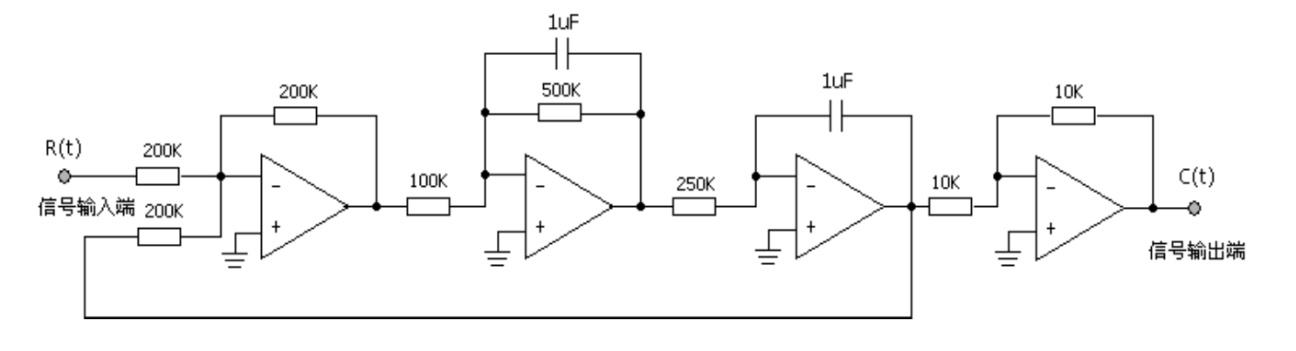
\includegraphics[width=0.8\textwidth]{fig4-2_circuit_unc.png}
    \captionof{figure}{未校正系统模拟电路图}
    \end{center}

    \item 未校正系统传递函数\\
    开环传递函数：
    \[G(s) = \frac{20}{s(0.5s+1)}\]
    闭环传递函数：
    \[\Phi(s) = \frac{40}{s^2+2s+40}\]

    \item \textbf{①求取校正前动态性能$t_s、\sigma\%$（误差带$\Delta=0.02$），并通过实物实验验证：}
标准二阶系统：
\[\Phi(s)=\frac{\omega_n^2}{s^2+2\zeta\omega_n s+\omega_n^2}\]
对比参数：
\[\omega_n=\sqrt{40}\approx6.32\ \text{rad/s},\quad 2\zeta\omega_n=2\Rightarrow\zeta\approx0.158\]
超调量：
\[\sigma\%=e^{-\pi\zeta/\sqrt{1-\zeta^2}}\times100\%\approx60.8\%\]
调节时间（$\Delta=2\%$）：
\[t_s=\frac{4}{\zeta\omega_n}=4\ \text{s}\]

    \item \textbf{②绘制校正前系统波特图，分析原始频域特性。}
\end{enumerate}

\textbf{(2) 校正装置的设计}
\begin{enumerate}
    \item 设计有源超前校正装置，设计指标：校正后开环剪切频率$\omega_c=20\ \mathrm{rad/s}$，相角裕度$\gamma\approx45^\circ$，绘制校正装置原理示意图；
    \item 超前校正装置传递函数：
    \[G_c(s) = \frac{0.5s+1}{0.05s+1}\]

    \item 校正装置模拟电路
    \begin{center}
    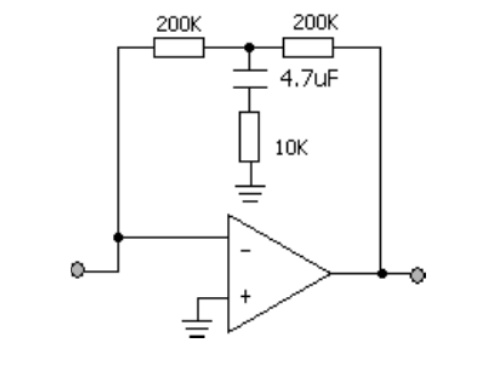
\includegraphics[width=0.5\textwidth]{fig4-3_circuit_corrector.png}
    \captionof{figure}{超前校正装置模拟电路图}
    \end{center}

    \item 已校正系统方框图
    \begin{center}
    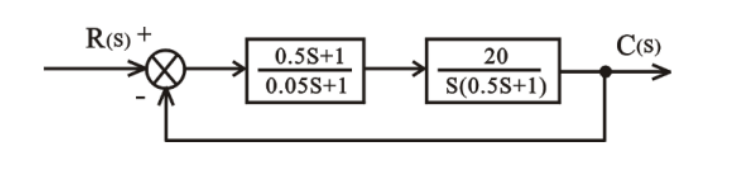
\includegraphics[width=0.7\textwidth]{fig4-4_block_corr.png}
    \captionof{figure}{校正后系统整体方框图}
    \end{center}
\end{enumerate}

\textbf{(3) 已校正系统}
\begin{enumerate}
    \item 已校正系统模拟电路图
    \begin{center}
    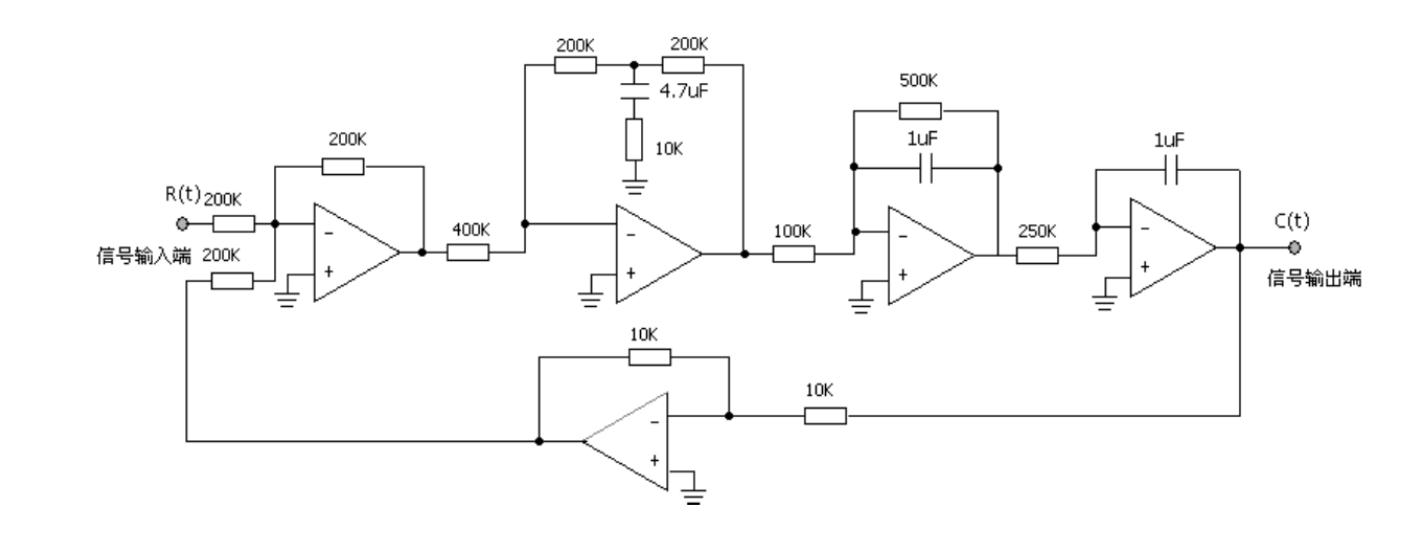
\includegraphics[width=0.9\textwidth]{fig4-5_circuit_corr.png}
    \captionof{figure}{校正后系统模拟接线电路图}
    \end{center}

    \item 已校正系统传递函数\\
   开环传递函数：
    \[G(s) = \frac{400}{s(s+20)}\]
    闭环传递函数：
    \[\Phi(s) = \frac{400}{s^2+20s+400}\]

    \item \textbf{①计算校正后$t_s、\sigma\%$理论值（$\Delta=0.02$），实验实测验证；}
对比标准二阶系统：
\[\omega_n=20\ \text{rad/s},\quad 2\zeta\omega_n=20\Rightarrow\zeta=0.5\]
超调量：
\[\sigma\%=e^{-\pi\zeta/\sqrt{1-\zeta^2}}\times100\%\approx16.3\%\]
调节时间（$\Delta=2\%$）：
\[t_s=\frac{4}{\zeta\omega_n}=0.4\ \text{s}\]

    \item \textbf{②实测开环频域指标$\omega_c、\gamma$，与理论计算值对比；}
    \item \textbf{③实测闭环时域$t_s、\sigma\%$，对标理论指标。}
\end{enumerate}

\noindent\textbf{注意事项：}
实验采集频率特性曲线时，启用配套上位软件「实验4 线性系统的频率响应实验」；实物接线前断电，防止短路损坏实验板运放元件。

\subsection{四、结合实验，并回答问题}
\paragraph{说明：按实验指导书要求完成四道思考题作答。}
\textbf{1. 二阶系统采用 PI 和 PD 控制性能上有何差别？}\\
答：
\begin{itemize}
    \item \textbf{PI 控制}：积分环节消除系统稳态误差，但引入相位滞后，降低系统相角裕度，系统超调变大、动态平稳性变差；
    \item \textbf{PD 控制}：微分项提供相位超前补偿，抬升相角裕度、抑制超调、加快响应速度，但缺少积分项，无法消除系统稳态误差。
\end{itemize}

\textbf{2. 二阶系统采用 PI 控制是否能兼顾动态响应的快速性和平稳性？为什么？}\\
答：不能兼顾。PI控制器内含积分环节，引入固定相位滞后，会降低系统相角裕度；若减小积分作用提升平稳性，系统无法消除稳态误差；增大积分消除静差则相位滞后加剧、振荡超调上升，无法同时满足快速与平稳。

\textbf{3. PI/PID 控制的 I 型系统（对象含一个积分环节）是否一定存在超调？为什么？}\\
答：不一定。I型仅保证阶跃输入无稳态误差，动态特性由控制器零极点配置决定；合理整定PI参数可使闭环系统全部极点落在s平面负实轴，系统处于过阻尼工作状态，实现无超调单调阶跃响应。

\textbf{4. 试凑法整定PID参数的大致步骤？}\\
答：
\begin{enumerate}
    \item \textbf{先比例：}令 $K_I=0,\ K_D=0$，单独调整$K_P$至系统出现临界小幅振荡；
    \item \textbf{再加积分：}接入$K_I$消除稳态误差，同步小幅下调$K_P$，补偿积分带来的稳定性衰减；
    \item \textbf{后微分：}引入$K_D$抑制动态超调，优化系统响应速度；
    \item \textbf{整体微调：}三个参数往复细调，综合满足超调、调节时间、稳态误差三项指标。
\end{enumerate}

\subsection{五、实验波形与数据结果}

\subsubsection{5.1 未校正系统实验波形}
\begin{figure}[htbp]
    \centering
    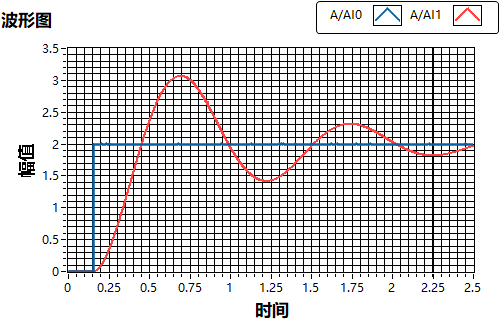
\includegraphics[width=0.32\textwidth]{1.1.png}
    \hfill
    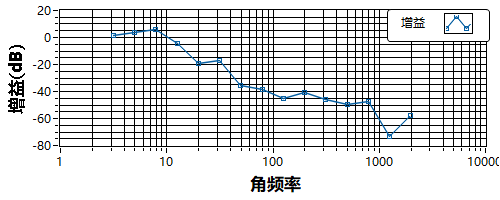
\includegraphics[width=0.32\textwidth]{1.2.png}
    \hfill
    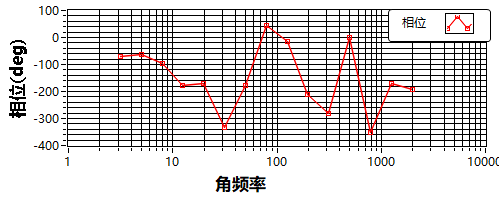
\includegraphics[width=0.32\textwidth]{1.3.png}
    \caption{未校正：阶跃响应、幅频特性、相频特性曲线}
\end{figure}

\subsubsection{5.2 已校正系统实验波形}
\begin{figure}[htbp]
    \centering
    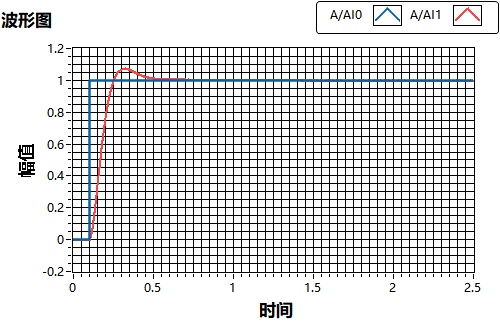
\includegraphics[width=0.32\textwidth]{2.1.png}
    \hfill
    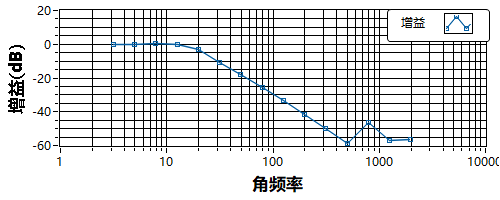
\includegraphics[width=0.32\textwidth]{2.2.png}
    \hfill
    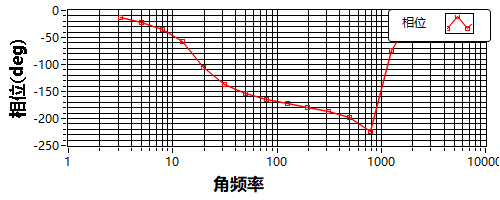
\includegraphics[width=0.32\textwidth]{2.3.png}
    \caption{校正后：阶跃响应、幅频特性、相频特性曲线}
\end{figure}

\subsubsection{5.3 实验数据记录与对比表}
\begin{table}[h]
\centering
\zihao{-4}
\renewcommand{\arraystretch}{1.5}
\caption{实验数据记录与对比表}
\begin{tabular}{|c|c|c|c|c|}
\hline
\textbf{系统类型} & \textbf{指标} & \textbf{理论值} & \textbf{实测值} & \textbf{相对误差} \\
\hline
\multirow{4}{*}{未校正系统}
& 超调量 $\sigma\%$ & 60.8\% & 57.2\% & 5.92\% \\
\cline{2-5}
& 调节时间 $t_s$(s) & 4.0 & 4.28 & 7.00\% \\
\cline{2-5}
& 剪切频率 $\omega_c$(rad/s) & $\approx6.32$ & 5.98 & 5.38\% \\
\cline{2-5}
& 相角裕度 $\gamma$ & $\approx14.1^\circ$ & $14.9^\circ$ & 5.67\% \\
\hline
\multirow{4}{*}{已校正系统}
& 超调量 $\sigma\%$ & 16.3\% & 17.5\% & 7.36\% \\
\cline{2-5}
& 调节时间 $t_s$(s) & 0.40 & 0.435 & 8.75\% \\
\cline{2-5}
& 剪切频率 $\omega_c$(rad/s) & 20.0 & 18.95 & 5.25\% \\
\cline{2-5}
& 相角裕度 $\gamma$ & $45^\circ$ & $47.6^\circ$ & 5.78\% \\
\hline
\end{tabular}
\end{table}

\subsection{六、实验结果与分析}
本次实验采用有源超前校正方案对二阶I型被控对象做频域校正，从理论计算、MATLAB仿真与实物NI采集结果可见：未校正系统阻尼比偏小，超调量大、调节时间长、相角裕度偏低，动态性能较差；串联超前校正装置后，校正环节在中频段提供正相位补偿，系统相角裕度与截止频率同步提升，超调、调节时间大幅下降，动态指标满足预先设计要求。

实测数据和理论计算存在小幅误差，误差来源包含：①实验板电阻、电容标称参数与实际元件容差；②NI采集卡采样精度、接线引线寄生电感电容；③环境工频噪声、输入信号幅值偏差；④人工读取波特图坐标带来读数误差。整体变化规律与频域校正理论完全吻合，验证了超前校正依靠相位超前优化系统动态性能的基本原理。

\end{document}